\newpage
\section{Errori}
Durante l'utilizzo dell'applicazione QuizziPedia è possibile che l'utente incappi in alcuni errori presentati a video:

\label{Errore}
\begin{figure}[ht]
	\centering
	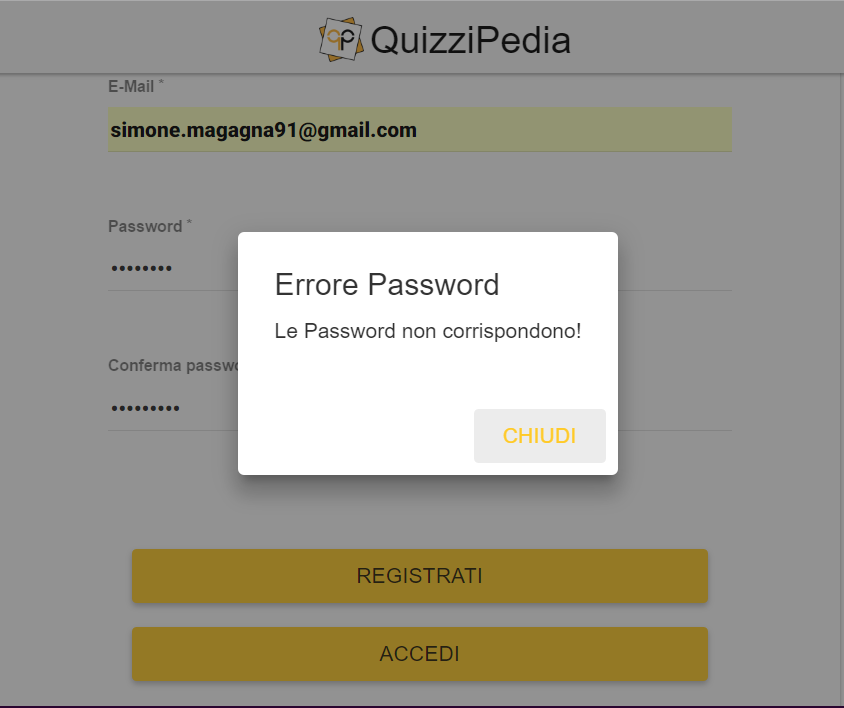
\includegraphics[scale=0.45]{img/errore.png}
	\caption{Errore: password non corrispondono}
\end{figure}
\FloatBarrier 

Viene ora presentata una lista contenente tutti i tipi di errore, con annessa descrizione, che un utente può trovare:

\begin{itemize}
	\item \texttt{Utente non trovato:} l'identificativo utente fornito non è un identificativo valido;
	\item \texttt{Credenziali non valide:} è necessario fornire un username ed una password valide;
	\item \texttt{Password assente:} è necessario inserire una password;
	\item \texttt{Password troppo corta:} è necessario inserire una password di almeno 8 caratteri;
	\item \texttt{Password uguale all'attuale:} è necessario inserire una password diversa della precedente;
	\item \texttt{Le password non coincidono:} è necessario che 'password' e 'conferma password' siano identiche;
	\item \texttt{Campo obbligatorio vuoto:} è necessario riempire tutti i campi obbligatori;
	\item \texttt{Username non disponibile:} l'username è già stato utilizzato, prego inserire un nuovo username;
	\item \texttt{Username non valido:} l'username non è valido;
	\item \texttt{Indirizzo mail non valido: } è necessario fornire un indirizzo e-mail valido;
	\item \texttt{Formato immagine non valido: } il formato dell'immagine non è valido;
	\item \texttt{Immagine di dimensione troppo grande: } la dimensione massima per l'immagine è di 20MB;
	\item \texttt{Caricamento immagine fallito}: errore sconosciuto nel caricamento dell'immagine;
	\item \texttt{Domanda non valida:} l'identificativo della domanda fornita non è un identificativo valido;
	\item \texttt{Argomento non valido:} l'identificativo dell'argomento fornito non è un identificativo valido;
	\item \texttt{Questionario non valido:}  l'identificativo del questionario fornito non è un identificativo valido;
	\item \texttt{Sommario non valido:} l'identificativo del sommario fornito non è un identificativo valido;
	\item \texttt{Contenuto domanda non valido:} i dati relativi al contenuto della domanda non sono  validi o sono formattati in modo errato;
	\item \texttt{Argomento non valido:} i dati relativi al contenuto dell'argomento non sono validi;
	\item \texttt{Contenuto questionario non valido:} i dati relativi al contenuto del questionario non sono validi;
	\item \texttt{Contenuto sommario non valido:} i dati relativi al contenuto del  sommario non sono validi o sono formattati in modo errato;
	\item \texttt{Dati modifica domanda non definiti:} i dati per la modifica di una domanda non sono definiti;
	\item \texttt{Argomento non definito:} i dati per la gestione dell'argomento non sono definiti;
	\item \texttt{Dati gestione questionario non definiti:} i dati per la gestione del questionario non sono definiti;
	\item \texttt{Sommario non valido:} i dati per la gestione del sommario non sono validi;
\end{itemize} 